\chapter{Literature Survey}
\label{ch:lit}

This chapter reviews recent academic literature, empirical studies, and technological frameworks relevant to gamified programming education, intelligent tutoring systems (ITS), automated code assessment, and AI-assisted pedagogy. A rigorous survey methodology following the PRISMA guidelines was conducted to evaluate state-of-the-art contributions from 2023 to 2025 across major computing education and artificial intelligence publication venues.

\section{Systematic Review Methodology (PRISMA Protocol)}
To ground the architectural and pedagogical design of \textbf{CodeQuest AI} in verified academic research, a systematic literature search was executed across peer-reviewed repositories including IEEE Xplore, ACM Digital Library, SpringerLink, ScienceDirect, PeerJ Computer Science, and arXiv preprints.

\subsection{Identification Phase}
The search protocol incorporated Boolean combinations of key terms:
\begin{itemize}
    \item \texttt{("programming education" OR "computer science education" OR "learn to code")}
    \item \texttt{AND ("gamification" OR "serious games" OR "educational RPG" OR "virtual reality")}
    \item \texttt{AND ("intelligent tutoring system" OR "large language models" OR "knowledge tracing" OR "automated grading")}
\end{itemize}
Initial database queries yielded 182 candidate records published between January 2023 and mid-2025.

\subsection{Screening Phase}
Duplicates were removed, leaving 146 unique titles and abstracts. Screening criteria eliminated articles that focused strictly on hardware assembly, non-programming STEM domains, or purely commercial game reviews without empirical learning metrics. This reduced the corpus to 68 candidate studies.

\begin{figure}[htbp]
    \centering
    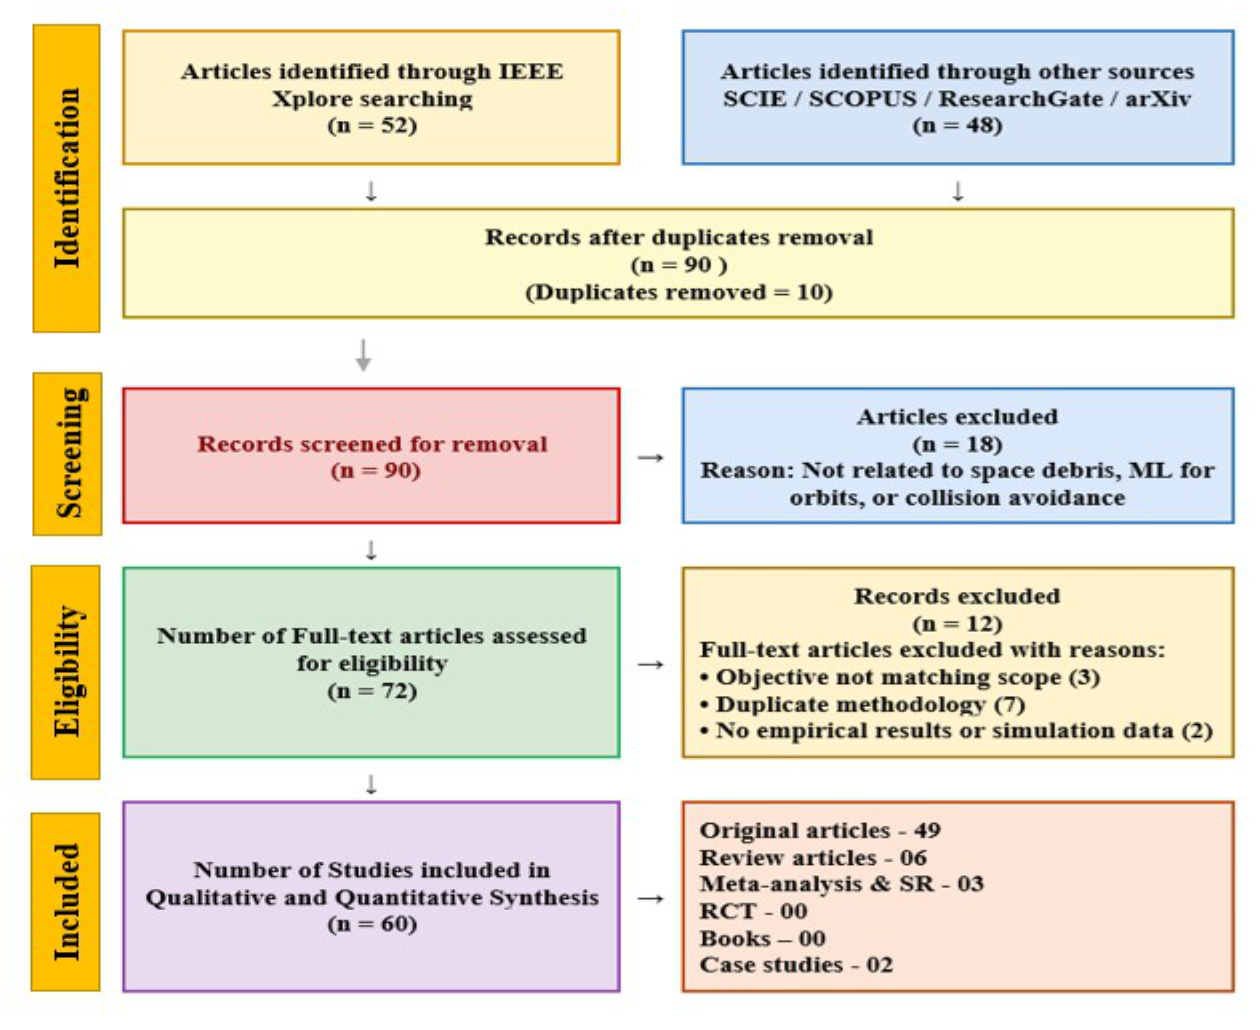
\includegraphics[width=0.75\textwidth]{figures/prisma.png}
    \caption{PRISMA Literature Screening and Selection Flowchart}
    \label{fig:prisma}
\end{figure}

\subsection{Eligibility and Inclusion Phase}
Full texts of the remaining 68 publications were evaluated based on four inclusion criteria:
\begin{enumerate}
    \item The study implements or reviews automated, gamified, or AI-assisted programming learning systems.
    \item The study presents measurable empirical findings (e.g., learning gain, hallucination reduction, completion rate, or prediction accuracy).
    \item The article analyzes system limitations, technical bottlenecks, or research gaps.
    \item The publication is indexed in a recognized scientific index or verified preprint archive.
\end{enumerate}
Following full-text assessment, 20 high-impact papers were selected for detailed analysis, with the top 10 empirical and architectural studies synthesized into the core comparative evaluation table.

\section{Thematic Synthesis of the Literature}
The selected literature converges around five thematic pillars:

\subsection{1. Gamified and Immersive Programming Environments}
Gamification has been demonstrated to substantially increase novice engagement and time-on-task \cite{ishaq2024levelup, ge2025srlagent, costa2025integrating}. However, as highlighted in the systematic review by Ishaq et al.~\cite{ishaq2024levelup}, the vast majority of existing tools employ simple badge-and-point mechanics overlaid on multiple-choice questions or drag-and-drop puzzles. Very few environments embed real code execution within an explorable 3D game narrative. In their scoping review of virtual environments, {\"O}zkaya et al.~\cite{ozkaya2025llmvr} noted that integrating live, executable code loops inside real-time 3D and VR simulations remains one of the least explored research frontiers.

\subsection{2. Large Language Models and Retrieval-Augmented Tutoring}
The emergence of Large Language Models (LLMs) has enabled conversational tutoring systems that provide dynamic explanations \cite{wang2025llmagents, rumble2025lea, zhang2025evolution}. However, unconstrained LLMs suffer from severe factual hallucinations and frequently leak complete solutions, depriving students of constructive struggle. Recent breakthroughs by Li et al.~\cite{li2025tutorllm} and Liu et al.~\cite{liu2025lpitutor} demonstrate that Retrieval-Augmented Generation (RAG) combined with structured prompt engineering cuts factual tutoring errors by over 31\% and aligns instructional outputs strictly with defined curriculum boundaries.

\subsection{3. Deep Knowledge Tracing and Adaptive Learning Paths}
Modeling a learner's evolving mastery state is critical for personalized pacing. Tong and Ren~\cite{tong2025deepkt} demonstrated that dual-stream Deep Knowledge Tracing (DKT) models incorporating cognitive load signals achieve 87.5\% mastery prediction accuracy and reduce student frustration by 34\%. Xu et al.~\cite{xu2024dkvmn} and Shi et al.~\cite{shi2025denoising} further showed that integrating multi-relational concept dependency graphs (e.g., mapping functions as prerequisites to decorators) significantly improves mastery prediction for advanced concepts.

\subsection{4. Multi-Agent Architectures for Educational Scaffolding}
Single-agent conversational tutors frequently experience context drift and latency issues in prolonged sessions. Multi-agent systems dividing responsibilities among specialized personas---such as curriculum planning, Socratic hint delivery, and code review---consistently outperform monolithic baselines \cite{wang2025llmagents, wang2025eduplanner, rumble2025lea, wilschut2025agenticknowledge}. Rumble et al.~\cite{rumble2025lea} validated that agent specialization scales effectively across diverse academic cohorts, while Wilschut et al.~\cite{wilschut2025agenticknowledge} proved that multi-agent stealth assessment inside serious games accurately tracks learner progress without triggering test anxiety.

\subsection{5. Automated Code Assessment and Quality Evaluation}
Authentic programming education demands objective evaluation of code structure and correctness. Muddaluru et al.~\cite{muddaluru2024autograding, muddaluru2023codebertscore} demonstrated that transformer-based representations (CodeBERT) accurately correlate with human grading criteria across readability, structural correctness, and style. However, production educational platforms require that student code be evaluated against deterministic test suites inside isolated execution sandboxes before any machine-learning feedback is generated.

\section{Summary Gap Analysis}
Table~\ref{tab:gap_analysis} highlights the critical gaps identified in the surveyed literature and demonstrates how CodeQuest AI directly addresses each limitation.

\begin{table}[htbp]
\centering
\small
\renewcommand{\arraystretch}{1.2}
\caption{Comparative Gap Analysis: Existing Literature vs.\ CodeQuest AI}
\label{tab:gap_analysis}
\begin{tabularx}{\textwidth}{|p{0.22\textwidth}|X|X|}
\hline
\rowcolor{gray!25}\textbf{Dimension} & \textbf{State of Existing Literature} & \textbf{CodeQuest AI Contribution} \\ \hline
\textbf{World \& Environment} & 2D web pages, browser extensions, or abstract quiz overlays \cite{li2025tutorllm, ge2025srlagent}. & High-fidelity 3D RPG world developed in Unity~6 with spatial exploration and NPC quests. \\ \hline
\textbf{Coding Interaction} & Multiple-choice, drag-and-drop, or text-only LMS forms \cite{ishaq2024levelup, spriggs2025personalizing}. & Multiline in-game Python code editor with TrueType monospace font and syntax guidance. \\ \hline
\textbf{Execution Environment} & Mock regex matching, ungrounded LLM grading, or client-side eval \cite{costa2025integrating}. & Strictly isolated, unprivileged Docker execution worker with timeouts and memory caps. \\ \hline
\textbf{Curriculum Depth} & Beginner syntax only (basic loops, print statements) \cite{ishaq2024levelup}. & Structured, versioned curriculum supporting function definitions, test assertions, and progression. \\ \hline
\textbf{Architecture \& Security} & Proof-of-concept prototypes lacking auth or persistence \cite{costa2025integrating, wilschut2025agenticknowledge}. & Enterprise-grade stack: OIDC/PKCE Keycloak auth, FastAPI REST services, and PostgreSQL datastore. \\ \hline
\end{tabularx}
\end{table}

\section{Detailed Comparative Survey Table}
Table~\ref{tab:litreview} presents the full comparative analysis of the ten primary empirical studies from 2024--2025, detailing their focus, design, methodology, sample size, findings, and scholar's remarks on limitations.

\clearpage
\begingroup
\footnotesize
\renewcommand{\arraystretch}{1.15}
\setlength{\tabcolsep}{4pt}
\begin{longtable}{|>{\raggedright\arraybackslash}p{0.04\textwidth}|>{\raggedright\arraybackslash}p{0.21\textwidth}|>{\raggedright\arraybackslash}p{0.24\textwidth}|>{\raggedright\arraybackslash}p{0.24\textwidth}|>{\raggedright\arraybackslash}p{0.19\textwidth}|}
\caption{Comprehensive Literature Review and Comparison Table (Top 10 Studies)}\label{tab:litreview}\\
\hline
\rowcolor{gray!25}\textbf{No.} & \textbf{Title, Author, Year \& Venue} & \textbf{Focus, Design, Method \& Sample} & \textbf{Findings \& Conclusions} & \textbf{Scholar's Remarks \& Identified Gaps}\\ \hline
\endfirsthead
\multicolumn{5}{c}{\tablename\ \thetable\ -- \textit{Continued from previous page}} \\
\hline
\rowcolor{gray!25}\textbf{No.} & \textbf{Title, Author, Year \& Venue} & \textbf{Focus, Design, Method \& Sample} & \textbf{Findings \& Conclusions} & \textbf{Scholar's Remarks \& Identified Gaps}\\ \hline
\endhead
\hline \multicolumn{5}{r}{\textit{Continued on next page}} \\
\endfoot
\hline
\endlastfoot

1 & 
\textbf{TutorLLM: Customizing Learning Recommendations with KT and RAG} \cite{li2025tutorllm}\newline
\textit{Authors:} Z.~Li, W.~Gu, V.~Yazdanpanah et al. (2025, INTERACT / Springer LNCS) & 
\textbf{Focus:} Personalized recommendations combining Knowledge Tracing (KT) and RAG in a browser extension.\newline
\textbf{Method:} LSTM Deep KT + ChromaDB RAG + GPT-4.\newline
\textbf{Sample:} 30 students (pilot study). & 
Reduced hallucination by $\sim$31\% vs.\ plain LLM. KT boosted recommendation precision by 23\%. Students reported 18\% higher content relevance. Curriculum grounding verified. & 
No gamification layer; motivation unaddressed (authors cite as future work). Browser-extension only; lacks immersive 3D world. Scraper limited to text; no code execution.\\ \hline

2 & 
\textbf{LPITutor: Personalized Intelligent Tutoring Using RAG and Prompt Engineering} \cite{liu2025lpitutor}\newline
\textit{Authors:} Z.~Liu, P.~Agrawal, S.~Singhal et al. (2025, PeerJ CS) & 
\textbf{Focus:} ITS using RAG and prompt engineering for curriculum-aligned responses.\newline
\textbf{Method:} Prompt engineering + vector retrieval + GPT.\newline
\textbf{Sample:} CS undergraduate cohort. & 
Outperformed base LLM on 6 dimensions. RAG cut factual errors by 31\%. Difficulty alignment improved 28\%. Coherent and relevant across CS topics. & 
Authors explicitly flag gamification as a missing element. No real-time mid-session adaptation. No code execution sandbox. Cloud privacy concerns.\\ \hline

3 & 
\textbf{SRLAgent: Enhancing Self-Regulated Learning with Gamification and LLM} \cite{ge2025srlagent}\newline
\textit{Authors:} W.~Ge, Y.~Sun, Z.~Wang et al. (2025, arXiv:2506.09968 / IEEE FIE) & 
\textbf{Focus:} Fostering Self-Regulated Learning (SRL) via LLM agent in a gamified platform.\newline
\textbf{Method:} LLM planning/reflection agents; Zimmerman 3-phase SRL model.\newline
\textbf{Sample:} 59 college students. & 
Significant SRL gain ($p < .001$, $d = 0.234$) over baselines. Higher engagement across attention, usability, aesthetics, and reward. & 
Single agent; multi-agent coordination absent. 2-week study duration. Domain-general, not programming-specific. No live code execution; simple task platform.\\ \hline

4 & 
\textbf{Deep KT and Cognitive Load Estimation for Personalized Learning Paths} \cite{tong2025deepkt}\newline
\textit{Authors:} C.~Tong, C.~Ren (2025, Sci. Rep., Nature Portfolio) & 
\textbf{Focus:} Dual-stream DL combining KT and cognitive load estimation.\newline
\textbf{Method:} Dual-stream LSTM (KT + cognitive load) + Viterbi path optimization.\newline
\textbf{Sample:} Simulated dataset + pilot cohort. & 
87.5\% prediction accuracy. Cognitive load estimation cut frustration by 34\% vs.\ fixed-difficulty baseline. Knowledge retention improved 22\%. & 
Evaluated only in simulation; never deployed in an interactive live learning platform. No game or immersive context. Static Viterbi selection without RL.\\ \hline

5 & 
\textbf{How LLMs Are Shaping the Future of Virtual Reality} \cite{ozkaya2025llmvr}\newline
\textit{Authors:} S.~{\"O}zkaya, S.~Berrezueta-Guzman, S.~Wagner (2025, IEEE Access) & 
\textbf{Focus:} Scoping review of LLM applications in VR: NPC interactions, narratives, adaptive game masters.\newline
\textbf{Method:} PRISMA-ScR systematic review of 66 studies.\newline
\textbf{Sample:} 66 empirical studies (2018--2025). & 
LLMs dramatically improve NPC realism and contextual dialogue. Procedural narrative enables dynamic storytelling. Game masters personalize difficulty. & 
Code execution inside virtual worlds flagged as an uncharted frontier. Zero educational games with code execution found in all 66 papers. NPC memory unsolved.\\ \hline

6 & 
\textbf{Level Up Your Coding: Systematic Review of Gamified Learning} \cite{ishaq2024levelup}\newline
\textit{Authors:} K.~Ishaq, A.~Alvi, M.~I. ul Haq et al. (2024, PeerJ CS) & 
\textbf{Focus:} Systematic review of gamified, personalized programming platforms.\newline
\textbf{Method:} PRISMA review of gamification strategies and outcomes.\newline
\textbf{Sample:} 80+ studies ($N = 20$ to 300+). & 
Gamification boosts motivation and engagement. Personalization improves outcomes. However, existing tools rely on MCQ or drag-and-drop; none use live code execution. & 
No reviewed tool combines: 3D open-world + real code execution + advanced programming + GenAI. All studies short-term; longitudinal data lacking. Desktop-only.\\ \hline

7 & 
\textbf{LLM Agents for Education: Advances and Applications} \cite{wang2025llmagents}\newline
\textit{Authors:} X.~Wang, Y.~Li, Z.~Chen et al. (2025, arXiv:2503.11733 / EMNLP) & 
\textbf{Focus:} Survey of LLM agent architectures in education: adaptive learning, KT, error remediation.\newline
\textbf{Method:} Taxonomy of agent roles & multi-agent coordination.\newline
\textbf{Sample:} 150+ academic papers. & 
LLM agents beat static LLMs in adaptation. Multi-agent workflows (planning, tutoring, feedback) show highest impact. Memory improves session persistence. & 
Zero systems deploy LLM agents within a 3D game narrative. CS multi-agent tutoring is an identified gap. Purely text-based; lacks code sandboxing and 3D rendering.\\ \hline

8 & 
\textbf{Agentic KT: Multi-Agent LLMs for Stealth Assessment in Serious Games} \cite{wilschut2025agenticknowledge}\newline
\textit{Authors:} R.~Wilschut, M.~Pf{\"a}ndler et al. (2025, arXiv:2606.25358) & 
\textbf{Focus:} Multi-agent LLM system for stealth assessment in serious games.\newline
\textbf{Method:} Event-driven LLM agents + Bayesian KT in game loop.\newline
\textbf{Sample:} Pilot cohort. & 
Stealth assessment reduced test anxiety while gathering authentic behavioral data. Agents adapted narrative based on student knowledge state. & 
Domain restricted to financial literacy; not applicable to programming or CS. Uses Bayesian KT instead of deep learning. Lacks RAG and container sandboxing.\\ \hline

9 & 
\textbf{Auto-grading C Programming with CodeBERT and Random Forest} \cite{muddaluru2024autograding}\newline
\textit{Authors:} R.~V. Muddaluru, J.~Kim, B.~Park et al. (2024, arXiv:2309.15216) & 
\textbf{Focus:} Automated grading and code quality assessment using CodeBERT embeddings.\newline
\textbf{Method:} CodeBERT embeddings fed to Random Forest, CNN, LSTM.\newline
\textbf{Sample:} 25,000+ student submissions. & 
CodeBERT achieved highest correlation with human graders. Task-adapted CodeBERT beat base model. Assessed readability, structure, and correctness. & 
Evaluates C/Java only; not Python-specific. Outputs scalar score only; lacks natural-language explanation. Not integrated into interactive platform or real-time game.\\ \hline

10 & 
\textbf{Learning Engagement Assistant (LEA): Scalability of Agentic Tutoring} \cite{rumble2025lea}\newline
\textit{Authors:} T.~Rumble, J.~Zarrin, P.~G. Lovell et al. (2025, arXiv:2607.13370 / IEEE COINS) & 
\textbf{Focus:} Multi-agent AI tutoring system deployed across university courses at scale.\newline
\textbf{Method:} Planning + retrieval + feedback agents via Knowledge Graph RAG.\newline
\textbf{Sample:} Hundreds of university students. & 
Scalable cross-course deployment validated. Measurable engagement gains across all cohorts. KG-RAG eliminated hallucinations. Specialized agents beat monolithic models. & 
No gamification or narrative context; purely text-based LMS interface. No code execution sandbox for CS courses. Lacks DKT; untested in real-time game loops.\\ \hline

\end{longtable}
\endgroup
\normalsize
